\section{Incrementally maintain classifiers}
%road map
In this section, some recent works on incrementally maintaining materialized classifier parameters in database are presented, which initially originates from \cite{deshpande2006mauvedb} and follows by \cite{koc2011incrementally}. Both \cite{deshpande2006mauvedb} and \cite{koc2011incrementally} develop a system (MauveDB vs Hazy) to store typical statistical model parameters as database view in RDBMS and update the views incrementally when raw data are modified.   

\subsection{MauveDB}
%brief description to MauveDB
MauveDB primarily deals with wireless sensor network applications, where data are collected through underlying sensors, fitted with typical statistic model such as regression-based model and interpolation-based model and used for estimating missing or future results. The statistic models learned with those raw data are materialized as {\em model-based views}, which are created with a high-level SQL-like language. Due to the addition or removal of the sensors, raw data are updated constantly, which requires efficient view maintenance strategies. The details of how {\em model-based views} are defined, updated and queried for prediction are provided as follows, which highly depend on the types of statistical model.

\subsubsection{Basic notations}
We will use capitalized letters (e.g. $H$) to denote matrix, capitalized bold letters (e.g. $\textbf{T}$) to denote tables, lowercase letters (e.g. $x$ and $y$) to denote scalar value, bold lowercase letters (e.g. $\textbf{x}$) to denote variables or attributes in the table, letters with bar (e.g. $\bar{w}$) to denote a vector, $f(*)$ to denote functions ($*$ represents arguments of function $f$). Besides, we use $H_{i,j}$ to denote the value at cell $(i,j)$ in matrix $H$ and use $\bar{w}_i$ to denote $i_{th}$ element in vector $\bar{w}$. We introduce superscript $^{(t)}$ (e.g. $x^{(t)}$) to denote the value of certain variables at the time step $t$ during iterative computation. Based on those notations, we provide notations for each model as follows.

\paragraph{Regression model}
A regression model is usually written as the following form:
\begin{equation}
t=\sum_{i=1}^kw_ih_i(*)
\end{equation}
where $h_i$ represents {\em basis function}, which is a monomial of {\em predictor variables} while $w_i$ represents coefficient of those monomials and $t$ is the {\em response variable}.

For example, in wireless sensor network application, temperature is measured at a 2D-space with coordinate $x$ and $y$, which can be computed with the following typical polynomial of the two predicator variables:

\begin{equation}
temp=w_1 + w_2x+w_3x^2 + w_4y+w_5y^2
\end{equation}
where the basis functions are $\{h_1(x,y), h_2(x,y), h_3(x,y),h_4(x,y), h_5(x,y)\}=\{1, x, x^2, y, y^2\}$

Given a set of data observed from the underlying wireless sensors located at different positions, $\{x_j,y_j,temp_j\}(j=1,2,\dots,n)$, the coefficients $\bar{w}^* = \{w_1,w_2,\dots,w_k\}$ are estimated with the following linear system:
\begin{equation}\label{eq: regression_solve}
    H^TH\bar{w}^*=H^T\bar{f}
\end{equation}

where $H$ is:
\begin{equation}
    H=\begin{bmatrix}
h_1(x_1,y_1) & h_2(x_1,y_1) &\dots &h_k(x_1,y_1)\\
h_1(x_2,y_2) & h_2(x_2,y_2) &\dots &h_k(x_2,y_2)\\
\dots\\
h_1(x_n,y_n) & h_2(x_n,y_n) &\dots &h_k(x_n,y_n)
\end{bmatrix}
\end{equation}

and $\bar{f}$ is:

\begin{equation}
    \bar{f} = \{temp_1, temp_2,\dots, temp_n\}^T
\end{equation}

In general, $H$ will be a matrix which represents data sets of $n$ data points with $k$ features while $\bar{f}$ represents the label vectors.

\paragraph{Interpolation model} 

The goal of interpolation is to estimate missing values of response variables given a value of predictor variable, which does not exist in the set of existing value pair for predictor variable and response variable. Specifically, given a variable pair $(\textbf{t},\textbf{v})$ and a set of value pairs for those two variables, $(t_i, v_i)(i=1,2,\dots,n)$ observed from sensors are then used to estimate value $v'$ of variable $V$ given a value $t'$ of variable $T$ $(t_j< t' < t_{j+1})$. Usually, {\em linear interpolation} is used. So $v'$ is estimated with value pair $(t_j, v_j)$ and $(t_{j+1}, v_{j+1})$ as follows:
\begin{equation}\label{eq: interpolation}
    v'= v_j + (v_{j+1}-v_j)\times\frac{t'-t_j}{t_{j+1}-t_j}
\end{equation}




\subsubsection{View definition}

MauveDB developed an declarative SQL-like language for users to define model-based view, which is exemplified in Figure \ref{fig:MauveDB_view_def}. Although different models cannot be manipulated in exactly the same way due to their different characteristics, the commonalities are still leveraged in this language. 

In Figure \ref{fig:MauveDB_view_def}, examples of regression-based view and Interpolation-based view definitions are presented in (i) and (ii) respectively. Same as way to create other database views, the view schemas, where the raw data comes from to construct the views (represented by \textit{SELECT}, \textit{FROM}) and what conditions the raw data should satisfy (represented by \textit{WHERE}) should be declared in the view definition statements. The model types (\textit{FIT} and \textit{INTERPOLATE} for regression and interpolation respectively) should be also specified along with partitions of raw data on each of which the models are trained (\textit{FOR EACH}) and other model-related information (such as base function for regression model, represented by \textit{BASE}). After executing statements shown in Figure \ref{fig:MauveDB_view_def}, {\em model-based views} are then created and stored in the RDBMS as relational tables.


\begin{figure}
    \centering
    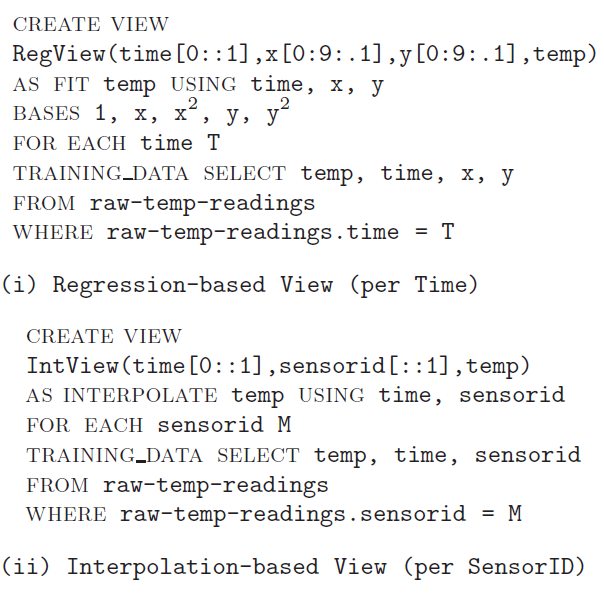
\includegraphics[width=8cm, height=8cm]{Figures/MauveDB_create_view.png}
    \caption{Define views in MauveDB}
    \label{fig:MauveDB_view_def}
\end{figure}

\subsubsection{View maintenance}
%High-level descriptions of view maintenance strategies
When the new data are available, the updates should be reflected on the model-based views. Four different strategies are developed for this purpose and their trade-offs are discussed with extensive experiments. The details of the four view maintenance strategies are introduced in this section.

\textit{Strategy 1: Materialize the views (eager approach)}
A naive way is simply to construct the models and materialize the model parameters as views in the database, which can avoid unnecessary query execution time when users want to retrieve the ``exact'' model information. However, such views may incur high space overhead and pose a challenge in refreshing the model as new data comes.

\textit{Strategy 2: Always use the base data }
This strategy goes to another extreme without materialization at all in the database, which can obviously make query processing very expensive since recomputating the view content is necessary every time when queries are evaluated. 

\textit{Strategy 3: Partial materialization (lazy approach)}
Somewhere in-between is to partially materialize the view content, which simply caches parts of the views that have been computed by certain queries. When the views are about to be refreshed, the corresponding cached contents in memory will be invalidated.

\textit{Strategy 4: Materialize an intermediate representation}
Some intermediate representations are materialized in this strategy by leveraging some nice properties of regression model and interpolation model, which have been an efficient solution experimentally and are presented as follows for the two models respectively.

For regression model, recall that the optimal coefficients can be solved with Equation \ref{eq: regression_solve}. The intermediate representation for it can be simply the materialization of matrix $H^TH$ and $H^T\bar{f}$, which can be beneficial in various aspects. First, the dimensions of the two matrices only rely on the total number of features, which thus won't lead to large space overhead. Besides, efficient updates to the two matrices are achievable since they are computed with linear operators, i.e. matrix multiplications and additions. A newly generated data point $(x',y', temp')$ can trigger the update of $H^TH$ and $H^T\bar{f}$ as follows:
\begin{equation}
    (H^TH)^{new}_{i,j} = (H^TH)^{old}_{i,j} + h_i(x',y')*h_j(x',y')
\end{equation}
\begin{equation}
    (H^T\bar{f})^{new}_i = (H^T\bar{f})^{old}_i + h_i(x',y')*temp'
\end{equation}

Once the user queries arrive, the coefficient $\bar{w}$ is computed with the following expression:
\begin{equation}
    \bar{w}^*=(H^TH)^{-1}H^T\bar{f}
\end{equation}

which can be computed with time complexity $Q(k^3)$ where $k$ is the total number of features.

For interpolation model, following the example shown in Figure \ref{fig:MauveDB_view_def}, the data in the interpolation-based view $\textbf{V}$ will be of the form $(\textbf{t}, \textbf{v})$ where $\textbf{t}$ represents time while $\textbf{v}$ represents observed value by the sensors. Unlike regression mode, its intermediate representations are not additional data but some additional data structure for searching the values of variable $\textbf{t}$. In order to efficiently estimate the sensor values for time $t'$ which is missing from the view instance but queried by users, the closest values $t_{-}$ and $t_{+}$ (along with the corresponding sensor values $v_{-}$ and $v_{+}$) to $t'$ are retrieved with the auxillary data structure such that $t'$ lies in the interval $(t_{-}, t_{+})$ with no other $\textbf{t}$ value from $\textbf{V}$ in it. So the estimated sensor value at time $t'$ can be computed using Equation \ref{eq: interpolation}.

The specific choice of strategies in practice depends on various factors, such as the query workload, data statistics and types of models. The trade-off between the four strategies are experimentally explored with extensive experiments in \cite{deshpande2006mauvedb}, which shows that the strategy 4 performs best in most scenarios while strategy 1 can actually outperform others in some cases.

\subsection{Hazy}
Hazy is another system for incrementally maintaining classifiers in RDBMS, which extends and improves MauveDB in the following aspects. 1) more linear classifers are supported, including support vector machines, ridge regression and logistic regression; 2) both eager and lazy strategies used in MauveDB are optimized by speeding up the updates and read operations.

\subsubsection{Views in Hazy}
\begin{figure}
    \centering
    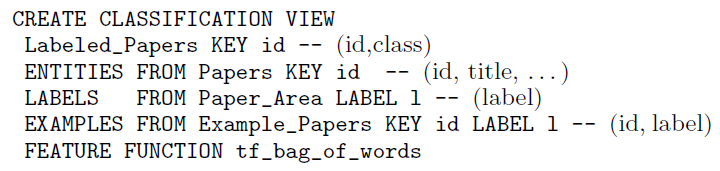
\includegraphics[width=10cm, height=2.5cm]{Figures/Hazy_view.png}
    \caption{Define views in Hazy}
    \label{fig:Hazy_view_def}
\end{figure}

%intro to view definition
In Hazy, users can declare views in the way shown in Figure \ref{fig:Hazy_view_def}, in which a {\em classification view} is defined over some entity table (i.e. $Papers$ in Figure \ref{fig:Hazy_view_def}, with Primary key $id$) to identify their type (i.e. $Paper\_area$) with a model trained using some training examples (i.e. $Examples\_papers$) that are derived from original entity table by applying some feature function (i.e. $tf\_bag\_of\_words$ function). So in the end, the content of the classification view is the classification results for the set of entities to be classified, in which each tuple has the form $(id, class)$ where $id$ is the entity id while $class$ is the label for that entity determined by the model. The major difference between eager and lazy strategies in terms of classification view definition is that the former one stores the materialized views in the database while the latter one only keeps views virtual.

%operations in Hazy and the bottleneck for eager and lazy approach
Hazy focus on three typical queries issued by the users: 1) {\em Single entity} read, i.e. retrieve the label of a single entity; 2) {\em All members} read, i.e. retrieve the labels for all the entities; 3) {\em Update}, i.e. update the views once new training examples arrive. Intuitively, the {\em update} should become the bottleneck for eager approach since the materialized views should be refreshed whenever updates happen while the {\em All members} read should be the major overhead for lazy approach since the content of the virtual views should be computed whenever read queries are issued, which are the major concerns for the authors of Hazy. In terms of {\em update} queries, the authors of Hazy assume that in the time to retraining the model is negligible (roughly on the order of 100$\mu$s on their datasets) and the major overhead is to relabel the entities in the materialized views for eager approach. 

\subsubsection{Overview of view maintenance in Hazy (eager approach)}
%overview of view maintenance problem
In this section, the details on how to maintain materialized classification views in Hazy are provided, which targets at more efficient {\em update} queries for eager approach rather than recomputing the content of views from the scratch when updates arrive. Lazy approach is free from this issue since updates won't influence the virtual views in the database. 

%introduce notation for table H
Suppose support vector machine is used thereafter (more complicated classifiers are introduce later) for binary classifications, at epoch $i$, the model parameters will be $(\bar{w^{(i)}}, b^{(i)})$. Given an entity with feature vector $\bar{f}$, its label is determined by the sign of the residual $eps = \bar{w^{(i)}}\cdot\bar{f}-b^{(i)}$. If $eps > 0$ ($eps < 0$ respectively), then this entity is labeled as $+$ ($-$ respectively).

Recall the assumption that the time to retrain the model is not significant, the model is firstly retrained at each epoch. Given the updated model parameters, a scratch table $\textbf{H}$ is maintained inside Hazy and varied across different epochs, which stores tuples of the form $(id, \bar{f}, eps)$ where $id$, $\bar{f}$ and $eps$ represents the entity id, feature vector and residual ($eps = \bar{w^{(i)}}*\bar{f}-b^{(i)}$). Then the classification view $\textbf{V}$ can be obtained from $\textbf{H}$, in which each view tuple has the form $(id, c, eps)$ ($c$ is the label for entity with identifier $id$ and is calculated as $c=sign(eps)$). For a tuple $t \in \textbf{H}$ ($\in \textbf{V}$), we use $t.attr$ denote the value of attribute $attr$ at tuple $t$ where $attr$ is an attribute of $\textbf{H}$ ($\textbf{V}$ respectively). For example, $t.\bar{f}$ and $t.id$ represent the feature vector and the entity at tuple $t$ in $\textbf{H}$.

%introduce two steps
\paragraph{Incremental step VS reorganization step} At epoch $i$, Hazy maintains table $\textbf{H}^{(s)}$ which is constructed at epoch $s$ ($s < i$), view $V^{(i+1)}$ can be either {\em incrementally} constructed from $V^{(i)}$ by updating small portion of view tuples in $V^{(i)}$ without changing $\textbf{H}^{(s)}$ or computed by referencing latest $\textbf{H}$ ({\em reorganized} at epoch $i$). Intuitively, the {\em incremental} step is relatively cheaper since it only touches parts of the view content, which, however, can incur more overhead when the model is far away from the model in the beginning as the time goes by. So the {\em reorganization step} is needed after applying the {\em incremental step} for some epochs to reduce the overhead in the following epochs to apply {\em incremental step}.

%cost of the two options
\paragraph{Cost measure and skiing strategy} In order to determine the optimal strategy on which step to take at each epoch, Hazy quantifies the cost for each of the two steps and formalizes it as the classic {\em ski rental problem}. In this problem, the cost of the {\em incremental option} is defined as the time to update $V^{(i)}$ to $V^{(i+1)}$, which should be proportional to the view tuples relabeled at epoch $i$ (denoted as $c^{(i)}$) while the {\em reorganization step} has a fixed cost $S$. Suppose the {\em reorganization step} is taken at epoch $s$, then the accumulated cost at epoch $i$ by applying {\em incremental step} since epoch $s$ is $a^{(i)} = \sum_{j=s+1}^ic^{(j)}$. The strategy to choose proper steps ({\em skiing strategy}) is as follows: If the accumulated cost $a^{(i)}$ is too large, say, greater than $\alpha S$ ($\alpha$ is a constant), then refreshing table $H$ is needed (the accumulated cost $a^{(i)}$ is reset to 0 after that). This strategy is proven to be 2-approximation asymptotically compared to the optimal strategy.


\subsubsection{Details of incremental step}\label{Sec: incremental step}
%overview
The core idea of {\em incremental step} is to do small changes to the classification view content to reflect the updates approximately, the details of which are presented as below. It starts by introducing how to determine which part of view tuples to be changed at each epoch with two thresholds, which follows by the detailed derivation rules of the two thresholds.

\paragraph{Thresholds in incremental step}
%intro to lower water and higher water
For incremental step, it is assumed that the appearance of the new training examples do not result in great changes to the model, which means that it is safe to simply update small portion of the view content to achieve performance gains at each epoch. Intuitively, the entities that are far away from the decision boundary should be less likely to be changed when the updates happen while the ones closer to the decision boundary are more likely to flip the labels. So Hazy introduces two thresholds, lower water and higher water (denoted by $lw$ and $hw$ respectively, which are negative and positive respectively) to determine which view tuples should be changed or not. At each epoch $i$, by referencing the residual value $eps$ for each entity in the scratch table $\textbf{H}^{(s)}$ computed at epoch $s$ ($s<i$), if $eps$ is greater than $hw$ (less than $lw$), then the labels of the corresponding entities are (highly likely to be) $+$ ($-$ respectively) and thus remain unchanged. Otherwise, we use the updated model at epoch $i$ to reclassify those entities. 

%how to compute lower water and higher water
\paragraph{How to determine the thresholds}
Intuitively, the two thresholds $hw$ and $lw$ should be adjusted at each epoch $i$ since the differences between model at epoch $i$ and model at epoch $s$ (when $\textbf{H}$ is recomputed) may be varied for different $i$. So $hw$ and $lw$ are associated with superscript $^{(s,i)}$ to indicate that they are related to the models at epoch $s$ and $i$, i.e. $hw^{(s,i)}$ and $lw^{(s,i)}$ respectively, which are computed as follows:

\begin{equation}
    lw^{(s,i)} = min_{l=s,\dots, i}\epsilon_{low}^{(s,l)},
    hw^{(s,i)} = min_{l=s,\dots, i}\epsilon_{high}^{(s,l)}
\end{equation}

where $\epsilon_{low}^{(s,l)}$ and $\epsilon_{high}^{(s,l)}$ are computed as (recall that $t.\bar{f}$ represents the feature vector of $t$):
\begin{equation}
    \epsilon_{low}^{(s,l)} = max_{t \in \textbf{H}}||t.f||_q||\bar{w^{(s)}}-\bar{w^{(l)}}||_p+b^{(s)}-b^{(l)}, \epsilon_{high}^{(s,l)} = - max_{t \in \textbf{H}}||t.f||_q||\bar{w^{(s)}}-\bar{w^{(l)}}||_p+b^{(s)}-b^{(l)}
\end{equation}
where the norm $q$ and $p$ satisfy $p^{-1} + q^{-1} = 1$


There is a nice property by applying Holder's inequality \cite{rudin1976principles} to $\epsilon_{low}^{(s,j)}$ and $\epsilon_{low}^{(s,j)}$, i.e. at epoch $j$, for a tuple $t \in \textbf{H}^{(s)}$, if $t.eps \geq \epsilon_{high}^{(s,j)}$ ($t.eps \leq \epsilon_{low}^{(s,j)}$), then $t.id$ should be in the class $+$ ($-$).

\subsubsection{Details of reorganization step}
The {\em reorganization step} for the scratch table $\textbf{H}$ includes recomputing the residual $\epsilon$ for each entity in $\textbf{H}$, reconstructing necessary indexes to quickly search the entity in $\textbf{H}$ and sorting the entire table by the residual $eps$, which happens when the current model is far away from the model computed in the last reorganization step. A greedy strategy is proposed earlier.  Formally speaking, when the cost of {\em reorganization step} (fixed as $S$, which is the time to perform the {\em reorganization step}) is less than the accumulated cost $a_{i}$, {\em reorganization step} is executed.

\subsubsection{Analysis of the greedy strategy}
Two assumptions about the cost measure are made when designing such greedy strategy: 1) the cost of incremental step, $c^{(s, i)}$ only depends on the current epoch $i$ and the most recent epoch $s$ for reorganization step since $c^{(s, i)}$ is a function of the number of tuples within the interval $[lw^{(s,i)}, hw^{(s,i)}]$; 2) Reorganization more recently won't increase the cost $c^{s,i}$, which means that $c^{(s, i)} < c^{(s',i)}$ for $s > s'$. The assumptions above can guarantee 2-approximation compared to theoretical optimal strategy. The analysis is sketched as follows.

%notations
Suppose during reorganization step, it takes $\sigma S$ to scan $\textbf{H}$. Given $N$ epochs in total, reorganization step is executed $M$ times, which happens at epoch $\mu_1, \mu_2,\dots, \mu_M$ ($0 \leq \mu_1 < \mu_2 < \dots < \mu_M \leq N$), The integer sequence $\bar{\mu} = \mu_1, \mu_2,\dots, \mu_M$is defined as a {\em schedule} under a certain strategy. At any epoch $i$, we define $\floor{i}_{\bar{\mu}} = max\{\mu \in \bar{\mu} | \mu < i\}$, which intuitively returns the most recent epoch before epoch $i$ when {\em reorganization step} is executed. Denote the set of costs for every epoch by $\bar{c} = \{c^{(s,i)}\}$, the total cost of a {\em schedule} will be:
\begin{equation}\label{eq: cost}
    Cost(\bar{\mu}, S, \bar{c}) = \sum_{i=1,2,\dots,N}c^{(\floor{i}_{\bar{\mu}}, i)} + MS
\end{equation}

Equation \ref{eq: cost} indicates that the total cost not only depends on how to schedule the reorganization step, but also depends on the cost at each epoch, i.e., $\bar{c}$ and $S$. This is because at each epoch, the value of $c^{(\floor{i}_{\bar{\mu}}, i)}$ is known to us only after the incremental step is over (recall that $c^{(s,i)}$ represents the execution time of incremental step), which can influence the accumulated cost $a^{(i)}$ and thus influence the decision at some point (recall that the decision at epoch $i$ depends on whether $a^{(i)}$ is greater than $\alpha S$). So given a strategy $\Phi$, the schedule $\bar{\mu}$ should be a function of $\bar{c}$, i.e. $\bar{\mu} = \Phi(\bar{c})$.

In order to prove that the skiing strategy is a 2-approximation strategy, the {\em competitive ratio} (denoted by $\rho$) is defined as below, which is a ratio between the cost of a strategy $\Phi$ and and the optimal cost:
\begin{equation}
    \rho(\Phi) = sup_{\bar{c}}\frac{Cost(\bar{\mu}, S, \bar{c})}{Cost(\bar{o}, S, \bar{c})}
\end{equation}


It is proven that $\rho(skiing) = (1+\alpha + \sigma)$ where $\alpha$ is the positive root of $x^2 + \alpha x - 1$ and for any other deterministic strategy, $\rho(\Phi) \geq (1+\alpha + \sigma)$. Specifically, when the number of entities goes to infinity, the time to scan $\textbf{H}$ table, i.e. $\sigma S$ should be approaching 0 (recall that $S$ is the reorganization time, which includes the time to sort $\text{H}$. The sorting time is more expensive than scanning time). In this case, $\alpha \rightarrow 1$ and thus $\rho(skiing) \rightarrow 2$.

\subsubsection{Overview of read queries in Hazy (lazy approach)}
%overview
In this section, how Hazy improves the performance on read queries, i.e. {\em single entity} read and {\em all members} read is presented. Recall that in eager approach, the classification views are materialized. So read queries are not a bottleneck here since the labels of either single entity or all the entities can be retrieved from the view instance directly. On contrast, only the virtual views are used in lazy approach, which may slow down the read queries since the view content should be generated on line. As a result, the authors focus on improve the performance of read queries (especially {\em all members} queries) for lazy approach.

Suppose a user wants to retrieve all the entities of the positive class, which is a typical {\em all members} query, in the naive solution, at a certain epoch $i$, all the entities need to be scanned to be labeled with the current model. However, in Hazy, not all the entities are read to respond to this query, which are achieved by referencing the scratch table $\textbf{H}^{(s)}$ (reorganized at epoch $s$, $s < i$), reading all the tuple $t$ satisfying $t.eps > lw^{(s,i)}$ from $\textbf{H}^{(s)}$ and simply labeling the entities satisfying $t.eps \in [lw^{(s,i)}, hw^{(s,i)}]$ (recall that entities with residual $t.eps > hw^{(s,i)}$ should be guaranteed to be in the positive class). 

Same as view maintenance problem in the last few sections for eager approach, there also exists a trade-off on whether the scratch table $\textbf{H}$ should be reorganized. For the read queries for the lazy approach, the greedy strategy is applied to determine when to do reorganization but with different cost measure to quantify the overhead of {\em incremental step}. Suppose it takes $S'$ seconds to read the entire entities, the number of real positive entities is $N_{+}$ and the number of entities above the low water $lw^{(s,i)}$ is $N_{R}$, then the cost of {\em all members} queries will be $c^{(i)} = \frac{N_{R}-N_{+}}{N_{R}}S$ and the accumulated cost is calculated as in Section \ref{Sec: incremental step}. Then the rest of the skiing strategy here is identical to the one used for eager approach.


\subsubsection{Other optimizations in Hazy}
Hazy also provides two types of system variants to achieve the performance enhancement. The first variant of Hazy is to maintain the classification views and the scratch table $\textbf{H}$ in memory (refered as Hazy-MM), which can be safely discarded when reorganizations happen since the model parameters will be recomputed at each epoch. The other one is to hybrid the main-memory structure and the on-disk structure to reduce the memory footprint. The performance trade-offs between the original system design and the two variants are explored experimentally.

\subsubsection{Extends to other machine learning models}
In the previous sections, it is assumed that the default machine learning algorithm is support vector machine and the problems Hazy is dealing with belong to binary classification problem. But Hazy is also flexible to handle other machine learning models (with kernel methods) and multi-class classification.

\paragraph{Other machine learning model}
Other linear classification model can be also supported by Hazy, which includes ridge regression and logistic regression. Actually, typical linear classification model can be formalized as {\em convex optimization problem} as below:

\begin{equation}\label{eq: opt_expr}
    min_{\bar{w}}P(\bar{w}) + \Sigma_{(\bar{x},y) \in \textbf{T}}L(\bar{w}\cdot\bar{x}, y)
\end{equation}

where $\bar{x}$ is the feature vector, $P$ is the {\em regularization term} and $L$ is the {\em loss function}. Typical solution to optimize the objective function shown in Equation \ref{eq: opt_expr} is to apply gradient descent methods to derive $\bar{w}$ iteratively until it converges to $\bar{w}*$, which is then used to classify a certain sample with feature values $\bar{x}$ as follows:
\begin{equation}
    l(\bar{x}) = h(\bar{w}\cdot\bar{x})
\end{equation}

where $h$ is simply sign function for binary classification problem.

Since the objective function of other linear classification models share the same form as support vector machine, it is pretty straightforward to migrate the solutions to those classification models.

\paragraph{Kernel methods}
Kernel methods extend linear classification models with kernel function $K: \mathbb{R}^d \times \mathbb{R}^d \rightarrow \mathbb{R}$, which is a positive semi-definite function. Given a kernel function, the corresponding classification function would be:
\begin{equation}\label{eq: kernel classification}
    l(\bar{x})=h(\Sigma_{i=1,2,\dots,N}c_i\cots K(\bar{s_i}, \bar{x}))
\end{equation}
where $\bar{s}_i$ is the {\em support vector} and $c_i$ is the weight value. In this case, the weight vector $\bar{w}$ is: $\bar{w} = \{c_1, c_2,\dots, c_N\}$, which can still fit the eager approach and lazy approach proposed before.

%linearized kernels
Some further improvements can be applied to a special type of kernel functions called shift-invariant kernels, which satisfy $K(x, y) = K(x-y)$ where $K$ is a kernel function and regarded as a simple function. Shift-invariant kernels includes many common kernels, such as the Gaussian and the Laplacian kernel. By applying {\em random non-linear feature vectors} \cite{rahimi2008random}, $K(x, y) \approx z(x)^Tz(y)$ where $z$ is a random map: $\mathbb{S}^d \rightarrow R^D$ (suppose $x, y \in \mathbb{S}^d$), which can thus simplify Equation \ref{eq: kernel classification} as below:
\begin{equation}
    l(\bar{x})=h(\Sigma_{i=1,2,\dots,N}c_i\cots K(\bar{s_i}, \bar{x})) = h(\Sigma_{i=1,2,\dots,N}c_i\cots z(\bar{s_i})^Tz(\bar{x}))=h(\bar{v}^Tz(\bar{x}))
\end{equation}

where $v=\sum_{i=1,\dots,N}c_iz(\bar{s_i})$. This technique can substantially reduce the dimension.

\paragraph{Multi-class classification}
Hazy builds a decision-tree-like structure to turn a multi-classification problem to binary classification problem.


\subsection{Discussion}


\section{Incrementally compute matrix programs}
Matrix operations are quite ubiquitous in modern data analysis tasks, which usually involve small incremental data analysis where the datasets are dynamic. To effectively propagate the input changes through the matrix operation program to the output, there are some efforts which consider matrix as views and accomplish the goal of incremental view maintenance. One example is Linview \cite{nikolic2014linview}, which targets at converting iterative programs with basic matrix manipulation primitives: matrix addition, multiplication, subtraction, transpose and inverse, into a {\em trigger program} and propagating the {\em delta expressions} via the trigger programs to derive the new output rather than re-evaluating from the scratch. In what follows, how the authors of \cite{nikolic2014linview} model the iterative programs with matrix operations, represent and propagate {\em delta expressions} and deal with typical linear algebra programs are elaborated respectively.

\subsection{Model the iterative programs}\label{sec: iterative_model}
Iterative computation is very common in data analysis programs, for which naive re-evaluation from the scratch in the case of data updates can incur high over head. Under the assumption that the iterative programs end after a fixed number of iteration steps (even after updates), Linview deals with delta expression propagation through the program under three different iterative models.

\paragraph{Linear model} The first iterative model is {\em linear model}, which simply updates the result at $k_{th}$ epoch based on the results at $(k-1)_{th}$ epoch. Given the input $A$, the output at epoch $k$ is computed as:

\[T_k=
\begin{cases}
f(A)& k=1\\
g(T_{k-1}, A) & k=2,3,\dots\\
\end{cases}
\]

\paragraph{Exponential model} In the {\em exponential model}, the output at $k_{th}$ epoch depends on the result at $(k/2)_{th}$ epoch, which has larger steps compared to {\em linear model}, i.e.:

\[
T_k=
\begin{cases}
f(A)& k=1\\
g(T_{k/2}, A) & k=2,4,8\dots\\
\end{cases}
\]

\paragraph{Skip model} {\em Skip model} lies in between, in which the step between the computed iterations is adjustable. Given a skip size $s$, the result before $s_{th}$ epoch is computed by {\em exponential model} and then the result after $s_{th}$ epoch is computed every $s_{th}$ iteration. The {\em skip model} is thus represented as:

\[
T_k=
\begin{cases}
f(A)& k=1\\
g(T_{k/2}, A) & k=2,4,8\dots,s\\
h(T_{k-s}, T_{s}, A) & k=s, 2s,\dots
\end{cases}
\]

\subsection{Incremental computation}
This subsection is centered around how Linview represent and propagate delta computation through the linear algebra program, which starts by introducing the incremental updates over matrix manipulation primitives. Matrix multiplications are frequently used in the following analysis, which is assumed to have time complexity $O(n^{\gamma})$ ($2\leq \gamma \leq 3$, varies for different algorithms)

\paragraph{Delta rules for basic matrix operations}
Given a matrix $A$ and a function $f(*)$, small changes $\Delta A$ to $A$ leads to the changes of output of $f(A)$ as: $\Delta_A(f) = f(A+\Delta A) - f(A)$. By following the properties of basic matrix operations, such as matrix addition, matrix multiplication and matrix inverse, the delta rule is shown as follows:

\begin{center}
    \begin{minipage}{0.4\textwidth}
      \begin{itemize}
        \item $\Delta_A(f_1 f_2) = f_2\Delta_A(f_1) + f_1\Delta_A(f_2)$
        \item $\Delta_A(f_1 \pm f_2) = \Delta_A(f_1) \pm \Delta_A(f_2)$
        \item $\Delta_A(\lambda f) = \lambda \Delta_A(f)$
        \item $\Delta_A(f^{-1}) = f(A+\Delta A)^{-1}-f(A)^{-1}$
      \end{itemize}
    \end{minipage}
  \end{center}

Note that for most update rules shown above, the time complexity is $O(n^2)$ while in general case, the delta derivation for matrix inverse has the same overhead as reevaluation from the scratch, which is much more expensive than $O(n^2)$. However, under the assumption that $\Delta A$ is relatively small than $A$ and thus have lower rank ($k$) than $A$ ($n$) where $k \ll n$, $\Delta A$ can be decomposed into multiplication of vectors and thus much cheaper for computation, which is called {\em factored form}. For example, given a rank-1 $\Delta A$ ($=\bar{u}\bar{v}^T$), by applying Sherman-Morrison formula \cite{press2007numerical}, $\Delta_A(\lambda f)$ can be written as:

\begin{equation}\label{eq: matrix_inverse}
\Delta_A(f^{-1}) = -\frac{f(A)^{-1}\bar{u}\bar{v}^Tf(A)^{-1}}{1+\bar{v}^Tf(A)^{-1}\bar{u}}
\end{equation}

\paragraph{Delta representation}
The overhead of incremental updates also relies on how to represent the delta. It has turned out that naive representations won't help even for very simple program with very minor changes. 

\begin{example}\label{eg: incremental_naive_update}
For example, consider the following program to compute $A^8$ for an $n\times n$ matrix $A$:

\begin{center}
    $B:= AA$\\
    $C:= BB$\\
    $D:= CC$
\end{center}

Given a small change $\Delta A$, such as an update to the entry $A_{i,j}$, $\Delta A_{i,j}$, which has overhead $O(1)$, by applying the delta rules for matrix multiplication mentioned above, $\Delta B$, $\Delta C$ and $\Delta D$ are represented as:

\begin{equation}\label{eq: delta_b}
    \Delta B = (\Delta A) A + A (\Delta A) + (\Delta A) (\Delta A)
\end{equation}
\begin{equation}\label{eq: delta_c}
    \Delta C = (\Delta B) B + B (\Delta B) + (\Delta B) (\Delta B)
\end{equation}
\begin{equation}\label{eq: delta_d}
    \Delta D = (\Delta C) C + C (\Delta C) + (\Delta C) (\Delta C)
\end{equation}
    


Computing $\Delta B$ only requires $O(n)$ operations since $(\Delta A) A$ and $A (\Delta A)$ only need to scale the $i_{th}$ row and $j_{th}$ column of $A$ by $\Delta A_{i,j}$ respectively, which takes $O(n)$ time while $(\Delta A) (\Delta A)$ only incurs $O(1)$ overhead. In the end, compared to original $B$, the changes caused by $\Delta B$ appear in the $i_{th}$ row and $j_{th}$ column of $B$.

Similarly, we can derive that $\Delta C$ requires $O(n^2)$ operations, which ends up with the full updates to the entire $C$. The effect of update propagation is shown in Figure \ref{fig:update_propagete}.

\begin{figure}
    \centering
    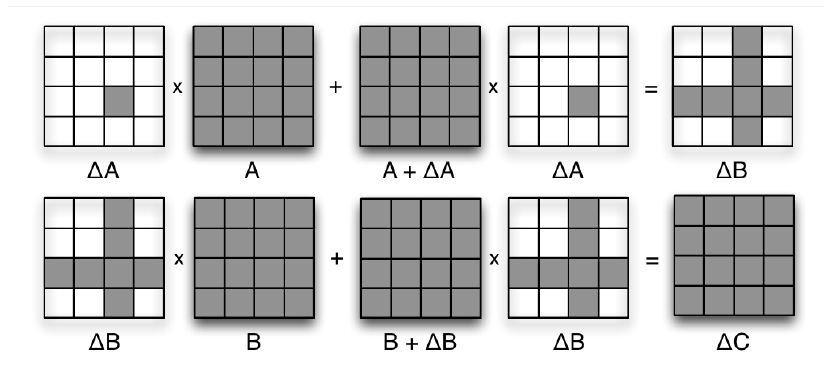
\includegraphics[width=10cm, height=4cm]{Figures/update_propagation.png}
    \caption{The effect of updates propagate}
    \label{fig:update_propagete}
\end{figure}

Then computing $\Delta D$ involves at least two full $O(n^{\gamma})$ matrix multiplications, which is obviously more expensive than recomputing $\Delta D$ from the scratch. \qed
\end{example}


To deal with this unexpected effect, the delta expressions are all represented as Example \ref{eg: incremental_naive_update} indicates, the updates $\Delta A$ is only a change to a single entry $A_{i,j}$, which is a rank-1 update and can be represented as $\Delta A = \bar{u}\bar{v}^T$ where $\bar{u}$ and $\bar{v}$ are both column vectors. Then by replacing $\Delta A$ in Equation \ref{eq: delta_b} with $\bar{u}\bar{v}^T$, $\Delta B$ is rewritten as:
\begin{equation}\label{eq: update_b_product}
\Delta B = \bar{u}(\bar{v}^TA) + (A\bar{u})\bar{v}^T + (\bar{u}\bar{v}^T\bar{u})\bar{v}^T=[\bar{u}, (A\bar{u}), (\bar{u}\bar{v}^T\bar{u})]
\begin{bmatrix}
    (\bar{v}^TA)  \\
    \bar{v}^T  \\
    \bar{v}^T   
\end{bmatrix}
=[\bar{u}_1, \bar{u}_2, \bar{u}_3]
\begin{bmatrix}
    \bar{v}^T_1  \\
    \bar{v}^T_2  \\
    \bar{v}^T_3  
\end{bmatrix}
\end{equation}

which is a sum of three outer products. The term $(\bar{v}^TA)$, $(A\bar{u})$ and $(\bar{u}\bar{v}^T\bar{u})$ can be all derived in $O(n^2)$ time while the vector $[\bar{u}, (A\bar{u}), (\bar{u}\bar{v}^T\bar{u})]$ and $[(A^T\bar{v}), \bar{v}, \bar{v}]$ are both $n \times 3$ matrices and thus the product of them requires $O(3n^2)$ operations.

In general, all the delta expressions can be expressed as a product of two $n \times k$ matrices where $k \ll n$, which only requires $O(kn^2)$ operations, although it is more expensive than naive updates for $\Delta B$ as shown in Example \ref{eg: incremental_naive_update}. For example, for $\Delta C$, since it is a sum of three products and each of them can be expressed as a product of two $n \times 3$ matrices by inserting Equation \ref{eq: update_b_product} to Equation \ref{eq: delta_c}, $\Delta C$ can thus be expressed as a a product of two $n \times 9$ matrices:


\begin{equation}
\begin{split}
    \Delta C &= (\Delta B) B + B (\Delta B) + (\Delta B) (\Delta B) \\&=[\bar{u}_1, \bar{u}_2, \bar{u}_3]
\begin{bmatrix}
    \bar{v}^T_1B \\
    \bar{v}^T_2B \\
    \bar{v}^T_3B 
\end{bmatrix}+[B\bar{u}_1, B\bar{u}_2, B\bar{u}_3]
\begin{bmatrix}
    \bar{v}^T_1 \\
    \bar{v}^T_2 \\
    \bar{v}^T_3 
\end{bmatrix}\\
&+[\bar{u}_1, \bar{u}_2, \bar{u}_3]
\begin{bmatrix}
    \bar{v}^T_1  \\
    \bar{v}^T_2  \\
    \bar{v}^T_3  
\end{bmatrix}
[\bar{u}_1, \bar{u}_2, \bar{u}_3]
\begin{bmatrix}
    \bar{v}^T_1  \\
    \bar{v}^T_2  \\
    \bar{v}^T_3  
\end{bmatrix}\\
&=[\bar{u}_1, \bar{u}_2, \bar{u}_3, B\bar{u}_1, B\bar{u}_2, B\bar{u}_3, \bar{u}_1, \bar{u}_2, \bar{u}_3]\\
&\begin{bmatrix}
    \bar{v}^T_1B \\
    \bar{v}^T_2B \\
    \bar{v}^T_3B \\
    \bar{v}^T_1  \\
    \bar{v}^T_2  \\
    \bar{v}^T_3  \\
    \bar{v}^T_1(\bar{u}_1\bar{v}^T_1 + \bar{u}_2\bar{v}^T_2 + \bar{u}_3\bar{v}^T_3)\\
    \bar{v}^T_2(\bar{u}_1\bar{v}^T_1 + \bar{u}_2\bar{v}^T_2 + \bar{u}_3\bar{v}^T_3)
    \bar{v}^T_3(\bar{u}_1\bar{v}^T_1 + \bar{u}_2\bar{v}^T_2 + \bar{u}_3\bar{v}^T_3)
\end{bmatrix}
\end{split}
\end{equation}

which requires $O(9n^2)$ operations in total. Finally, by inserting the expression of $\Delta C$ above into Equation \ref{eq: delta_d}, computing $D$ only requires $O(27n^2)$ operations, which is far cheaper than re-evaluation from the scratch.

Actually, $\Delta B$ can be further optimized as:
\begin{equation}\label{eq: update_b_product_opt}
\Delta B = \bar{u}(\bar{v}^TA) + (A\bar{u})\bar{v}^T + (\bar{u}\bar{v}^T\bar{u})\bar{v}^T=[\bar{u}, (A\bar{u}) + (\bar{u}\bar{v}^T\bar{u})]
\begin{bmatrix}
    (\bar{v}^TA)  \\
    \bar{v}^T 
\end{bmatrix}
=[\bar{u}_1', \bar{u}_2']
\begin{bmatrix}
    \bar{v}^T_1'  \\
    \bar{v}^T_2'  \\
\end{bmatrix}
\end{equation}

which is a product of two $n \times 2$ matrices. Consequently, $\Delta C$ and $\Delta D$ can be represented as a product of two $n \times 4$ matrices and two $n \times 8$ matrices respectively.

\paragraph{Constructing trigger functions}
Given the derivation rules above, Linview converts the linear algebra program into a set of trigger functions, which takes a set of input matrices and handle the updates of them sequentially. For example, given a set of input matrices $D=\{A, B, \dots\}$ and an evaluation function $f(*)$ over that, then the overall effect of updates will to $f(D)$ will be:

\begin{equation}\label{eq: updates_by_multi_vars}
\Delta_{D}(f(D)) = \Delta_{A}(f(D)) + \Delta_{D\\\{A\}}(f(D) + \Delta_{A}(f(D)))
\end{equation}


%  and Linview generates one trigger function for each of them, which is then used to monitor the change of the corresponding input matrix.

\subsection{Incremental analysis for typical programs}
The incremental update model above can fit some typical linear algebra programs, such as ordinary least squares, matrix powers and even more general forms, which are illustrated below.

\paragraph{Ordinary least squares}
Ordinary least squares is a classic regression problem, for which we need to derive the best parameter $\beta^*$ for a linear system, $Y = X\beta$ ($X$ is a $m \times n$ matrix representing predictors while $Y$ is a $m \times p$ matrix for response variables) through statistical estimates. With some typical statistic assumptions, such as Gaussian noise, the best estimates for $\theta$ is $\theta^* = (X^TX)^{-1}X^TY$.

In practice, the regression model is usually built in a dynamic environment where the incoming new data requires efficient model updates on the basis of the outdated model instead of computing from the scratch every time, for which the performance bottleneck is to update the inverse operation $(X^TX)^{-1}$. We represent $X^TX$ as $Z$. So given a rank-1 update to $X$, i.e. $\Delta X = \bar{u}\bar{v}^T$, $\Delta Z$ can be expressed as:
\begin{equation}
    \Delta Z = [\bar{v}\ \ (X^T\bar{u} + \bar{v}\bar{u}^T\bar{u})]\begin{bmatrix}
    \bar{u}^T X  \\
    \bar{v}^T  
\end{bmatrix}\\
=[\bar{p}_1\ \bar{p}_2]\begin{bmatrix}
    \bar{q}^T_1  \\
    \bar{q}^T_2  
\end{bmatrix}=\bar{p}_1\bar{q}_1^T + \bar{p}_2\bar{q}_2^T
\end{equation}

It has time complexity $O(mn)$ due to the computation of $X^T\bar{u}$, $\bar{v}\bar{u}^T\bar{u}$ and $\bar{u}^TX$, which ends up with a product of two $n\times 2$ matrices and thus a rank-2 update to $Z$. We can further $\Delta Z_1 = \bar{p}_1\bar{q}_1^T$ and $\Delta Z_2 = \bar{p}_2\bar{q}_2^T$ such that $\Delta Z_1$ and $\Delta Z_2$ are both rank-1 matrix. Considering the fact that both $X$ and $\Delta X$ are $m \times n$ matrices and thus $\bar{u}$ and $\bar{v}$ are $m \times 1$ and $n \times 1$ vector respectively, $\bar{p}_1$ and $\bar{q}_2$ should be both $n \times 1$ vectors. Besides, the computation result of $X^T\bar{u}$ and $\bar{v}\bar{u}^T\bar{u}$ are both $n \times 1$ vector and thus $\bar{p}_2$ (sum of $X^T\bar{u}$ and $\bar{v}\bar{u}^T\bar{u}$) should be also $n \times 1$ vector. Similarly, $\bar{q_1}^T$ is also $n \times 1$ vector.

By following Equation \ref{eq: matrix_inverse} and Equation \ref{eq: updates_by_multi_vars}, the update rules for $W = (X^TX)^{-1} = Z^{-1}$ with respect to $\Delta Z_1$ and $\Delta Z_2$ will be:

\begin{center}
\begin{equation}
\begin{split}
    \Delta_{Z_1}(W)& = -\frac{W\bar{p}_1\bar{q}_1^TW}{1 + \bar{q}_1^TW\bar{p}_1}\\
    \Delta_{Z_2}(W)& = -\frac{(W+\Delta_{Z_1}(W))\bar{p}_2\bar{q}_2^T(W+\Delta_{Z_1}(W))}{1 + \bar{q}_2^T(W+\Delta_{Z_1}(W))\bar{p}_2}
\end{split}   
\end{equation}
\end{center}

while simply computes the rank-1 update $\Delta Z_1$ to $W$ and then accumulate the effect of $\Delta Z_2$ for $W$. $\Delta_{Z_1}$ and $\Delta_{Z_2}$ can be further written as:

\begin{equation}
\begin{split}
\Delta_{Z_1}(W) = \bar{r}_1\bar{s}_1^T\\    
\Delta_{Z_2}(W) = \bar{r}_2\bar{s}_2^T
\end{split}
\end{equation}

where $\bar{r}_1 = W\bar{p}_1$, $\bar{r}_2 = (W+\Delta_{Z_1}(W))\bar{p}_2$ while $\bar{s}_1$ and $\bar{s}_2$ are the rest of the subexpressions of $\Delta_{Z_1}(W)$ and $\Delta_{Z_2}(W)$ respectively. So the overall updates to $W$ is $\Delta W = \bar{r}_1\bar{s}_1^T + \bar{r}_2\bar{s}_2^T$, which is a rank-2 update.
Since $\bar{p}_i$ and $\bar{q}_i$ ($i=1,2$) are column vector of length $n$ and $Z$ and $W$ are $n \times n$ matrices, the computation of $\bar{r}_1 = W\bar{p}_1$ thus need $O(n^2)$ operations, which is the same for $\bar{s}_1$, $\bar{s}_2$ and $\bar{r}_2$. So the overall cost to update $W$ is thus $O(n^2 + mn)$, which is far less than the cost of recomputing from the scratch, i.e. $O(n^3 + mn)$.

In terms of the update for $\beta^*$ (denoted by $\Delta \beta$), given the update to the input $X$, i.e. $\Delta X=\bar{u}\bar{v}^T$, $\Delta \beta$ can be thus written as:

\begin{equation}
    \Delta \beta = \Delta WX^TY + W\Delta X^TY + \Delta W\Delta X^TY = (\bar{r}_1\bar{s}_1^T + \bar{r}_2\bar{s}_2^T)X^TY + W\bar{v}\bar{u}^TY + (\bar{r}_1\bar{s}_1^T + \bar{r}_2\bar{s}_2^T)\bar{v}\bar{u}^TY
\end{equation}

while requires $O(n^2 + mp + np + mn)$ operations in total while re-evaluation incurs $O(mnp + n^2min(m,p))$ operations.

\paragraph{Matrix powers}
The goal of matrix powers is to compute $A^k$ for an input matrix $A$ with a given exponent $k$, which plays an important role in many data analysis tasks. Matrix powers can be computed iteratively, for which the three iterative models proposed in \ref{sec: iterative_model} is applicable and the trade-offs between the three models can be explored under re-evaluation strategy or incremental update strategy.

The time and space complexity of matrix powers under different iterative models and different evaluation strategies (re-evaluation or incremental update) is presented in Figure \ref{fig:time_space_complexity_matrix_power}. Under the assumption that $k \ll n$ 

\begin{figure}
    \centering
    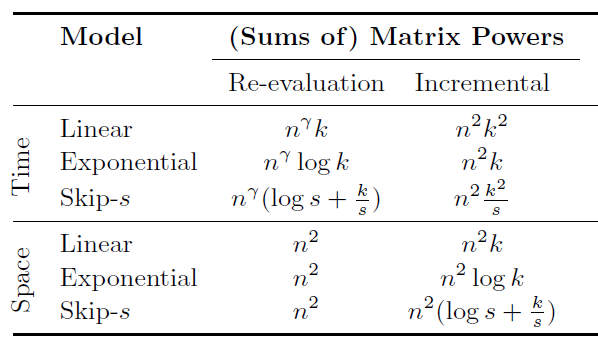
\includegraphics[width=8cm, height=4.5cm]{Figures/time_space_complexity_matrix_powers.png}
    \caption{The time and space trade-offs for matrix power}
    \label{fig:time_space_complexity_matrix_power}
\end{figure}

For re-evaluation strategy, it would require $O(n^{\gamma})$ operations for every iteration and thus the total time complexity depends on the number of iterations. Thus Exponential model outperform other models since it has largest leap between iterations. But all of the models have the same space complexity, i.e. $O(n^2)$.

For incremental update strategy, the computation time at each iteration should be $O(rn^2)$ where $r$ is the rank of the input delta expression on the updates at each iteration and the rank of delta expression increases linearly as the iteration proceed, which leads to the nearly quadratic running time and linear space consumption with respect to iteration number.

Similar to {\em matrix power}, the sum of matrix power problem, which aims at computing $S_k = I + A + A^2 + \dots + A^k$ given input $A$ and maximum exponent $k$ where $I$ is the identity matrix, have the almost the same computation process and thus have the same time complexity as shown in Figure \ref{fig:time_space_complexity_matrix_power}. 

\paragraph{General form} The authors also consider a general iterative matrix computation programs based on matrix powers, i.e. $T_{i+1} = AT_{i} + B$ where $A$ is the input matrix with dimension $n \times n$, $B$ is a constant matrix with dimension $n \times p$ and the result of $T_{i}$ is iteratively computed with dimension $n \times p$. Such general form appears in many applications such as PageRank and power iteration method for eigenvalue computation. 

Note that $T_{i+1} = AT_{i} + B$ can be unrolled as the form for computing $T_{i+k}$, i.e. $T_{i+k} = A^kT_{i} + (A^{k-1} + A^{k-2} + \dots + A + I) B$, in which how to efficiently incrementally compute $P_k = A^k$ and $S_k = (A^{k-1} + A^{k-2} + \dots + A + I)$ has been discussed before and thus both $P_k$ and $S_k$ are materialized and maintained along with $T_k$. Given those notations, the derivation rules for $T_{i+1} = AT_{i} + B$ under the three iterative models from Section \ref{sec: iterative_model} are shown in Table \ref{tab:derivation_rule}.

\begin{table}[]
    \centering
    \begin{tabular}{|c|c|}\hline
        Model & Derivation rule \\ \hline
        Linear & $T_k=
\begin{cases}
AT_0 + B& k=1\\
AT_{i-1} + B & k=2,3,4\dots,k
\end{cases}$\\ \hline
        Exponential & $T_k=
\begin{cases}
AT_0 + B& k=1\\
P_{i/2}T_{i/2} + S_{i/2}B & k=2,4,8\dots,s\\
\end{cases}$\\ \hline
        Skip-s &$T_k=
\begin{cases}
AT_0 + B& k=1\\
P_{i/2}T_{i/2} + S_{i/2}B & k=2,4,8\dots,s\\
P_sT_{i-s} + S_sB & k = 2s, 3s, \dots, k
\end{cases}$\\ \hline
    \end{tabular}
    \caption{Derivation rules for $T_{i+1} = AT_{i} + B$ under three iterative models}
    \label{tab:derivation_rule}
\end{table}

Then given an update $\Delta A$ against the input matrix $A$, the cost analysis under different iterative models and update strategies is provided below.

In terms of re-evaluation strategy, the results of $T_i$, $P_i$ and $S_i$ are only materialized for current iteration. For linear model, computing $AT_i$ is the performance bottleneck, which requires $O(np)$ operations (the result has dimension $n \times p$) with $O(n)$ multiplications for each operation. So the total time complexity is $O(pn^2)$ for each iteration and thus $O(pn^2)$ for $k$ iterations. For exponential model and skip-s model, maintaining $P_i$ and $S_i$ would incur time complexity $O(n^{\gamma})$ for every iterations, which is essential for $logk$ and $logs$ iterations respectively. Besides the cost of maintaining the auxiliary matrices $P_i$ and $S_i$, it still needs $O(pn^2)$ time to compute $P_sT_{i-s}$ or $P_{i/2}T_{i/2}$ at each iteration. Since the number of iterations for exponential model and skip-s model is $logk$ and $logs + \frac{k}{s}$ respectively, the overall time complexity for the two models will be $O(n^{\gamma} + pn^2)logk$ and $O(n^{\gamma}logs + pn^2(logs+ \frac{k}{s}))$.

For incremental strategy, the time complexity to maintain $P_s$ and $S_s$ is still $O(n^2)$ for each iteration as discussed before. To derive $T_k$, the update rule $P_{i/2}T_{i/2} + S_{i/2}B$ or $P_sT_{i-s} + S_sB$ is used, which requires extra $O(np)$ time to compute the factored form for $T_i$. So the overall time complexity for each iteration will be $O(n^2 + np)$. By following similar analysis for {\em matrix powers}, the time complexity and space complexity for the three different iterative models is presented in Figure \ref{fig:time_space_complexity_general_form}.

But notice that for some extreme case, such as $p=1$, incremental update strategy has worse performance than re-evaluation strategy, which is due to the unnecessary factor form representations for $T_i$ (a vector in this case). To solve this problem, a combination of the re-evaluation strategy and incremental updates strategy is proposed, which simply represent delta expression for $T_i$ as a single matrix instead of two factored vectors and still represent the auxiliary matrix $P_i$ and $S_i$ in factored form. So for exponential model and skip-s model, they require $rn^2$ operations to update $P_i$ and $S_i$ for each iteration where $r$ is the rank of them, which incurs the same overhead as the incremental updates for matrix powers while the time complexity to compute $T_k$ is $O(pn^2)$ when $P_i$ and $S_i$ are given, which has the same time complexity as re-evaluation strategy. By summing up the time complexity from the two parts, the overall time complexity is presented in Figure \ref{fig:time_space_complexity_general_form}. Since both $P_i$ and $S_i$ for hybrid strategy are materialized in the same form as incremental update strategy for every iteration, it thus shares the same space complexity as incremental update strategy.


\begin{figure}
    \centering
    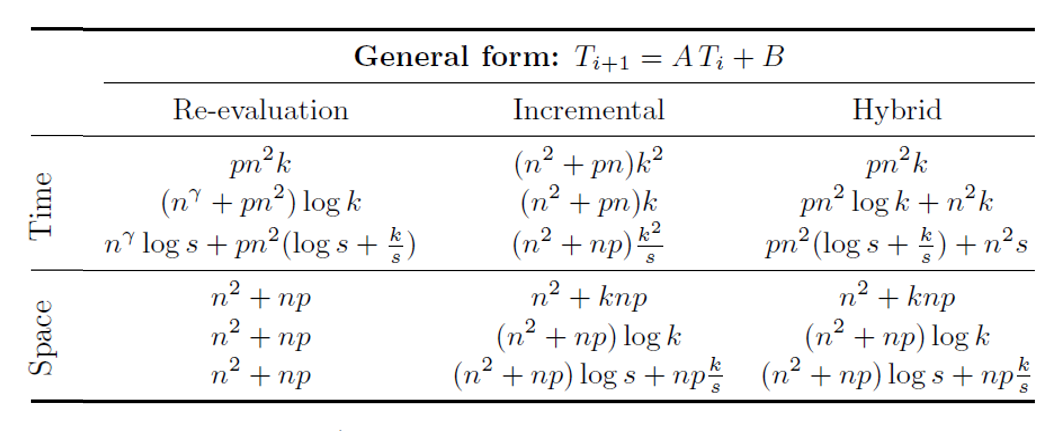
\includegraphics[width=12cm, height=4.5cm]{Figures/time_space_complexity_general_form.png}
    \caption{The time and space trade-offs for general forms}
    \label{fig:time_space_complexity_general_form}
\end{figure}


\subsection{Discussions}

\section{Incrementally derive new models with existing models}
In the last two sections, we reviewed related works on how to maintain views in the context of data analysis tasks, where the views can be the model parameters stored as tables in the RDBMS or matrices involved in linear algebra programs. However, given those predefined {\em views}, how to make their content usable for further data analysis tasks becomes another challenge, which is similar to traditional query rewriting using views problem where proper views are selected for answering queries \cite{halevy2001answering}.

In this section, \cite{hasani2018efficient} is introduced, which takes query optimization ideas to construct approximate machine learning models through {\em materialization} and {\em reuse}. The high-level idea of \cite{hasani2018efficient} is that user's issue a ``query'' on some tuples in a dataset for building a machine learning model, which is then approximately (but efficiently) constructed by reusing a set of pre-materialized models instead of from the scratch. When building the model to answer users' requests, \cite{hasani2018efficient} proposes two different approaches, i.e., {\em merging} the pre-materialized model parameters and constructing {\em coresets}, which incur different overhead and theoretical guarantee in terms of approximation but can deal with very general types of machine learning models, such as generalized linear models (GLMs), K-means and Guassian Mixture Models (GMMs).

In what follows, some basic concepts are introduced, which follows by the two approaches, {\em merging} and {\em coreset} approach along with an algorithm on how to find the minimal-cost strategy under some certain type of queries and some extensions in the end.


\subsection{Basic concepts}
The dataset that \cite{hasani2018efficient} is dealing with is a relation $\textbf{D}$ with $n$ tuples, $d$ attributes $\bar{\textbf{a}} = \{\textbf{a}_1, \dots, \textbf{a}_d\}$, which may have hierarchical structures (e.g. attribute $city$ with hierarchical structure $City \rightarrow State \rightarrow Country$) and can be divided into feature attributes $\bar{\textbf{x}}$ and labels attributes $\bar{\textbf{y}}$.

We can issue some queries to extract some tuples from $\textbf{D}$ via some predicates, such as {\em range based predicates} (e.g. $\textbf{a}_1 \in [lb, ub]$) and {\em dimension based predicates} (e.g. $\textbf{a}_2 = `c'$) over some attributes, which are then used for training a machine learning model. The entire approach has two phases, i.e. ``pre-computing phase'' and ``running time phase''. During ``pre-computing phase'', a set of pre-materialized machine learning models $\mathcal{M} = \{M_1, M_2, \dots, M_n\}$ are prepared for answering user query and each $M_i$ corresponds to a query predicate over $\textbf{D}$ which is used to extract tuples from $D$ to construct $M_i$. For example, given a relation $D=\{1,2,\dots, 1000\}$, the pre-materialized models $\{M_1, M_2, \dots, M_5\}$ can be built over the range predicate $P_1 = [1, 200], P_2 = [201, 400], \dots, P_5 = [801, 1000]$.
In the following ``running time phase'', given a user query with a predicate (e.g. $q=[250, 500]$), a set of candidate pre-materialized models are selected for approximately building the requested model.

As mentioned before, \cite{hasani2018efficient} targets at very general machine learning algorithms, such as K-means, GMMs and GLMs, the notations of which are briefly presented below:

\paragraph{K-means} K-means is an unsupervised clustering algorithm, which aims at computing a set of centroids $C$ from a set of data points $X$ and assigning each data point from $X$ to one of centroid in $C$ by minimizing the sum of square errors (SSE) with a similarity measure $d(*)$ in it:

\begin{equation}\label{eq: sse_k_means}
    SSE(X, C) = \sum_{\bar{x} \in X}d(\bar{x}, C)
\end{equation}

\paragraph{GMM} GMM is the probabilistic version of K-means, which is parameterized by a set of model parameters $\bar{\theta} = \{(w_1, \bar{\mu_1}, \Sigma_1), (w_2, \bar{\mu_2}, \Sigma_2), \dots, (w_k, \bar{\mu_k}, \Sigma_k)\}$ such that the probability of a data point $\bar{x}$ belonging to a cluster $i$ is computed by the probability density function of normal distribution and weighted by $w_i$, i.e.  $w_i\frac{exp(-\frac{1}{2}(\bar{x}-\bar{\mu}_i)^T\Sigma^{-1}(\bar{x}-\bar{\mu}_i))}{\sqrt{(2\pi)^k|\Sigma|}}$. The model parameters are derived during the training process with EM algorithm.

\paragraph{GLM} GLM includes a large class of typical linear classifiers such as logistic regression and support vector machine (SVM) and also typical regression methods, such as linear regression.

\subsection{Constructing models for user query}
In this subsection, assuming that there exists a set of pre-materialized models $\mathcal{M} = \{M_1, M_2, \dots, M_r\}$ built on different portions of $D$ and there is a user query $q$ over the subset of $D$, i.e. $D_q$, two approaches (i.e. {\em merging model} and {\em coreset construction}) used to obtain an approximate model $\tilde{M}_q$ for $q$ are presented below. 

\subsubsection{Constructing by merging models}
Suppose we can find a set of candidate pre-materialized machine learning models $\mathcal{M}_q (\subseteq \mathcal{M})$ usable for a user query $q$, {\em merging model} approach simply merges the parameters from each model in $\mathcal{M}_q$ to compute the parameters of the approximate model $\tilde{M}_q$, which varied across different machine learning algorithms.

\paragraph{Merging model for K-means}
For K-means, each pre-materialized model will store the centroids as the parameters. Suppose the union of the centroids from $\mathcal{M}_q$ is $C_w$ and the cluster represented by a centroid $c_j$ in $C_w$ includes $w_j$ data points from $\textbf{D}$. Then K-means++ \cite{arthur2007k} runs over $C_w$ with weight $w_j$ for each centroid $c_j \in C_w$ to produce k centroids as output, which will be a $O(log k)$-approximate model compared to the one constructed on $D_q$ directly and a $O(log^2k)$-approximate model compared to the optimial model on $D_q$.

\paragraph{Merging model for GMM}
The main takeaway of the solutions to K-means above is to clustering centroids from the candidate models with further invocations of the clustering algorithm, which, does not work for GMM, although GMM is a generalized model for K-means. This is because 1) the model parameters of GMM include mean vector, covariance matrix and a prior probability, which are far more complicated than K-means and far more expensive to estimate; 2) the merged model may be far away from the one built from the scratch. 

To overcome the issues above, the authors proposed an iterative approach to merge the GMM clusters from the candidate models $\mathcal{M}_q$, which starts by unioning all the cluster parameters from $\mathcal{M}_q$ (denoted by $\theta_q$) with the cluster parameters in the form of $(w_i, \bar{\mu}_i, \Sigma_i)$.
Then the most similar model pairs with parameters $(w_1, \bar{\mu}_1, \Sigma_1)$ and $(w_2, \bar{\mu}_2, \Sigma_2)$ are determined by Bhattacharyya distance \cite{bhattacharyya1943measure} (denoted by $D_B(*)$, see Equation \ref{eq: db_distance}), which are merged into a single cluster by following Equation \ref{eq: GMM_merging}.

\begin{equation}\label{eq: db_distance}
\begin{split}
    D_B(\bar{\mu}_1, \bar{\mu}_2, \Sigma_1, \Sigma_2) &=
    \frac{1}{8}(\bar{\mu}_1-\bar{\mu}_2)^T\Sigma^{-1}(\bar{\mu}_1 -\bar{\mu}_2) \\&+ \frac{1}{2}ln(\frac{|\Sigma|}{\sqrt{|\Sigma_1||\Sigma_2|}})\\
    \Sigma &= \frac{\Sigma_1 + \Sigma_2}{2}
\end{split}
\end{equation}

\begin{equation}\label{eq: GMM_merging}
    \begin{split}
        w &= w_1 + w_2\\
        \bar{\mu} &= \frac{1}{w}(w_1\bar{\mu}_1 + w_2\bar{\mu}_2)\\
        \Sigma &= \frac{w_1}{w}[\Sigma_1 + (\bar{\mu}_1 - \bar{\mu})^T(\bar{\mu}_1 -\bar{\mu})]\\
        &+\frac{w_2}{w}[\Sigma_2 + (\bar{\mu}_2 - \bar{\mu})^T(\bar{\mu}_2 -\bar{\mu})]
    \end{split}
\end{equation}

The merging process continues until there are exact k clusters in the end.


\paragraph{Merging model for classifiers}
Suppose for each model $M_i \in \mathcal{M}_q$, the model parameter is $\theta(M_i)$, in order to derive the approximate model $\tilde{M}_q$ for $q$, the model parameters from $\mathcal{M}_q$ are simply averaged, i.e. $\theta(\tilda{M}_q) = \frac{1}{|\mathcal{M}_q|}\Sigma_{M \in \mathcal{M}_q}\theta(M)$, which, however, has been proven by \cite{zhang2012communication} to match the error rate of the model built from the scratch on $D_q$.

\subsection{Answering query by coreset}
Merging model approach is very efficient since it constructs the approximate model for the user query without having to access the data points but it lacks theoretical guarantee compared to the model built from the scratch for some machine learning algorithms, which can be alleviated by coreset approach.

Specifically, a weighted set of data points $C \subseteq \textbf{D}$ is a $\epsilon-$coreset for $D \subseteq \textbf{D}$ if $C \subseteq D$ and $(1-\epsilon)\phi(D) \leq \phi(C) \leq (1+\epsilon)\phi(D)$ where $\phi$ is the loss function (e.g. Equation \ref{eq: sse_k_means}) and $\phi(D)$ and $\phi(C)$ are the evaluation of $\phi$ over $D$ and $C$. Intuitively, the coreset is a subset of $D$, $C$ such that the machine learning model built on (weighted) $C$ and $D$ are close enough.

Recall that there are two computation phases for constructing approximate model for user query, i.e. {\em pre-computing phase} and {\em running time phase}. In {\em pre-computing phase}, the coreset is constructed for every pre-materialized model while in {\em running time phase}, the coreset is used to construct approximate model for user query, which are illustrated below.

\paragraph{Coreset in pre-computing phase} The coreset is constructed during {\em pre-computing phase} by one common strategy, i.e. sampling the data points proportional to their ``importance'' to the loss function $\phi$. The ``importance'' is quantified by a surrogate function which should be selected to 1) have good approximation ratio compared to the loss function $\phi$; 2) guarantee efficient computation; 3) be  agnostic about the optimal solution computed by $\phi$. So the surrogate function should be varied across different machine learning algorithms. For example, for K-means with loss function shown in Equation \ref{eq: sse_k_means}, given a set of data points $D_i$, the surrogate function is defined as follow:

\begin{equation}\label{eq: surrogate_function}
    p(x) = \frac{1}{2}\frac{1}{|D_i|} + \frac{1}{2}\frac{d(x, \mu(D_i))^2}{\Sigma_{x'\in D_i}d(x', \mu(D_i))^2}
\end{equation}

where $\mu(*)$ is used to compute the mean of all $D_i$. This equation is efficient since it only requires two passes over the entire $D_i$ to compute the importance for every $x \in D_i$. After computing the probability for every data point in $D_i$, we can do the probability sampling over the data points from $D_i$, which guarantees that the result is $\epsilon-$coreset according to the proof in \cite{bachem2017scalable}.

\paragraph{Coreset in running time phase} There are two intriguing properties for coreset, which is beneficial to model construction in the running time phase. The first property is the {\em compositional} property, i.e. given the $\epsilon-$coresets $C_1$ and $C_2$ for two datasets $D_1$ and $D_2$, $C_1 \bigcup C_2$ should be also an $\epsilon-$coreset for $D_1 \bigcup D_2$, which can produce a coreset of large size for $D_q$ (the data points that the user query touches) if we union the coresets from all the candidate models from $\mathcal{M}_q$. 

To solve this issue, we employ the second property of coreset, i.e. the size of an $\epsilon-$coreset simply depends on $\epsilon$ and a probability value $\delta$ but independent from the dataset size. For example, with the probability $1-\delta$, to generate a $\epsilon-$coreset, which should have the size at least $\Omega(\frac{dk+log\frac{1}{\delta}}{\epsilon^2})$ where $k$ is the cluster number and $d$ is the dimension number. Suppose each model in $\mathcal{M}_q$ has a coreset of size $m$, by following this property, the coreset construction algorithm can be simply applied over the union of all the coresets from models in $\mathcal{M}_q$ (a set of size $m|\mathcal{M}_q|$) to generate a coreset of size $m$ for $D_q$.